% \begin{figure}
%     \centering
%     \includegraphics[scale=0.40]{figs/setup.jpg}
%     \caption{Suitcase-shaped mobile system with stereo camera and LIDAR}
%     \label{fig:setup}
% \end{figure}

%%%%%%%%% Feb 18 %%%%%%%%%

\begin{table*}[ht]
\centering
\caption {Video Datasets with egocentric viewpoint} \label{tab:data} 
\begin{tabular}{|P{0.25\textwidth}|P{0.25\textwidth}|P{0.25\textwidth}|P{0.25\textwidth}|} \hline
Dataset & Number of near-collision video sequences & Structure of scenes & Setup for recording \\ \hline 
\textbf{Ours} (Near-collision)  & 13,685 & Indoor hallways & Suitcase  \\ \hline 
UAV crashing \cite{gandhi} & 11,500 & Indoor hallways & UAV  \\ \hline  
DroNet \cite{DroNet} & 137 & Inner-city & Bicycle  \\ \hline 
%Collision trajectory \cite{ziebart} & 166 & Kitchen Area & Laser range finders & Fixed \\ \hline  
Robust Multi-Person Tracking \cite{Andreas} & 350  & Busy inner-city & Chariot \\ \hline   
\end{tabular}
\end{table*}

We sought to analyze a large-scale, real-world video dataset in order to understand challenges in prediction of near-collision events. However, based on our survey, existing datasets had a small number of interaction events as reported in Table \ref{tab:data} and lacked diversity in the capture settings. Therefore, in order to train robust CNN models that can generalize across scenes, ego-motion, and pedestrian dynamics, we collected an extensive dataset from a mobile perspective. Next, we describe our hardware setup and methodology for data collection. 
%We further provide the algorithm used for automatic ground truth annotation. 

\section{Hardware Setup}
The mobile platform used for data collection is shown in Fig.~\ref{fig:setup}, and includes a stereo camera and LIDAR sensor. While during inference we only utilize a monocular video, the stereo camera serves two purposes. First, it provides a depth map to help in automatic ground truth annotation. Second, it doubles the amount of training data by providing both a left and right image perspective which can be used as separate training samples. However, during the process of automatic data annotation, it was observed that the depth maps from stereo camera are insufficient for extracting accurate distance measurements. In particular, when the pedestrian is close to camera the depth values are missing at corresponding pixels due to motion blur. To resolve this issue we utilize a LIDAR sensor, which is accurate to within a few centimeters. The images and corresponding 3D point clouds are recorded at the rate of 10Hz.     

% The mobile platform shown in \ref{fig:setup} is used to collect videos inside university buildings. The data is split into train and test as follows:
% \begin{itemize}
% \item Training images - 10685 (2106 positive and 8579 negative)  
% \item Test images - 3563 (687 positive and 2876 negative)
% \end{itemize}
%  The camera and LIDAR are calibrated using \cite{calibration}. We used Faster RCNN object detector to detect the pedestrian in RGB image and recorded the ground truth position in world from projected point cloud. 

\section{Camera-LIDAR Extrinsic Calibration}
We use the camera and the LIDAR for automatic ground truth label generation. The two sensors can be initially calibrated with correspondences~\cite{Autoware,calibration}. An accurate calibration is key to obtaining the 3D position of surrounding pedestrians and annotating the large number of videos in our dataset. Let $R$ and $t$ denote the rotation matrix and the translation vector defining the rigid transformation between the LIDAR to the camera frame and $K$ the $3 \times 3$ intrinsic matrix of camera. Then, the LIDAR 3D coordinates $(x, y, z)$ can be related to a pixel in the image with coordinates $(U,V) = (\frac{u}{w}, \frac{v}{w})$ using following transformation:
%U = \frac{u}{w}; V = \frac{v}{w}
\begin{equation}\label{eq:Rt}
    \begin{bmatrix}u \\ v \\ w\end{bmatrix} = K[R \mid -R^{T}t] \begin{bmatrix} x \\ y \\ z \\ 1\end{bmatrix}
\end{equation}

Given this calibration, we can now project LIDAR points onto the image and obtain estimated depth values for the image-based pedestrian detection. 

%$$
%$$
%Here, . 
%% An example of projection of point cloud onto the image is shown in figure \ref{fig:projection}.
%% Show the pipeline - image showing projected point cloud, heatmap from GRADCAM 
%% Number of training and test images 

% \begin{figure}[h]
%     \centering
%     \includegraphics[scale=0.35]{figs/point_cloud_projected_over_image.eps}
%     \caption{Point cloud projected on image to extract 3D pose}
%     \label{fig:projection}
% \end{figure}


%For people detection, we employ a state-of-the-art person detection (Faster-R-CNN \cite{fasterRCNN}). Given a person detection, we can then compute its 3D location in the scene from the corresponding 3D point cloud.

%However, Autoware requires 30-40 poses of calibration target to output accurate transformation and thus we later shifted to \cite{calibration} which only requires 1-3 poses.  

\section{Large-Scale Data Collection and Annotation}
The platform is pushed through three different university buildings with low-medium density crowd. Our recorded videos comprise of cafeteria and hallways of varying styles. 
%Each image is automatically annotated with a binary label using algorithm \ref{algo}. 
%An illustration of the resulting processing is shown in Fig. \ref{fig:gt}. A positive binary label indicates the presence of humans within the radius of 1 meter around the setup. As presented in line 3 of algorithm \ref{algo}, we detect the persons' bounding boxes by applying Faster RCNN \cite{fasterRCNN} on image and thus the persons behind the setup are not considered. 
We experimented with several techniques for obtaining pedestrian detections in the scene from the image and LIDAR data. As 2D person detection is a well-studied problem, we found an image-based state-of-the-art person detection (Faster-R-CNN \cite{fasterRCNN}) to perform well in most cases, and manually inspect and complete any missing detections or false positives. To obtain the 3D position of each detected bounding box, we compute a median distance of its pixels using the 3D point cloud. An illustration of the resulting processing is shown in Fig. \ref{fig:gt}. Each image is annotated with a binary label where a positive label indicates the presence of at least one person within a meter distance from setup. We understand that the people in camera's view who move in the same direction as camera might not be important for collision. However, the number of such instances is insignificant in our dataset. \\
%Some of the halls also have students sitting on study tables who are also referred to as pedestrians in this paper.

% \begin{algorithm}
% \caption{Ground Truth Labeling}
% \label{algo}
% \begin{algorithmic}[1]
% \STATE \text{\textbf{Input:} A tuple of ($image_t, LIDAR_t$)}
% \STATE \text{\textbf{Init:} $label_{t} = 0$}
% \STATE \text{Bounding boxes $\leftarrow$ FasterRCNN($image_t$)}
% \FOR {\text{box in Bounding Boxes}}
% \STATE \text{distance inside box = $\emptyset$}
% \FOR {\text{point $[x, y, z]$ in $LIDAR_{t}$}}
% \STATE $\begin{bmatrix}u \\ v \\ w\end{bmatrix} = K[R \mid -R^{T}t] \begin{bmatrix} x \\ y \\ z \\ 1\end{bmatrix}$ \COMMENT{from Eq. \ref{eq:Rt}}
% \IF {$(\frac{u}{w}, \frac{v}{w})$ lies inside box}
% \STATE \text{add $\sqrt{x^{2} + y^{2}}$ to distance inside box}
% \ENDIF
% \ENDFOR
% \STATE \text{pedestrian distance = Median(distance inside box)}
% \IF {pedestrian distance $<$ 1 meter}
% \STATE \text{$label_{t} = 1$}
% \ENDIF
% \ENDFOR
% \STATE \text{return $label_{t}$}
% \end{algorithmic}
% \end{algorithm}

Now we want to estimate the time to near-collision, in terms of milliseconds, based on a short temporal history of few RGB frames. Let us consider a tuple of $N$ consecutive frames 
%$(image_{1}, image_{2}, \hdots, image_{N})$ 
$(I_{1}, I_{2}, \hdots, I_{N})$ and using this sequence as history we want to estimate if there is a proximity over the next 6 seconds. 
%Predictions farther than 6 seconds will largely be redundant while navigating in dynamic public places. 
Since the framerate is $10$ fps, we look at the next 60 binary labels in future annotated 
%using algorithm \ref{algo}
as $\{label_{n+1}, label_{n+2}, \hdots, label_{n+60}\}$. If we denote the index of first positive label in this sequence of labels as $T$ then our ground truth time to near-collision is $t = \frac{T}{10}$ seconds. 

\begin{figure}
    \centering
        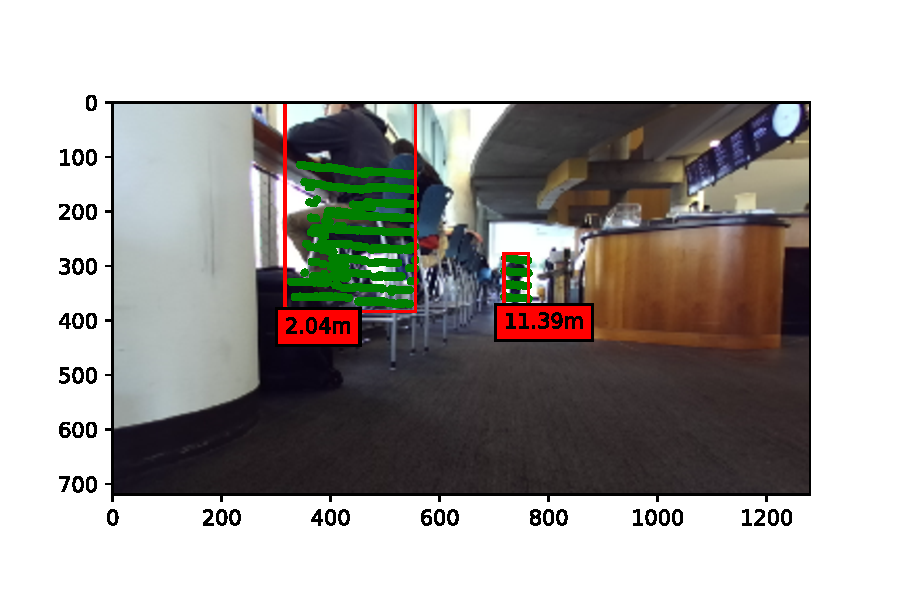
\includegraphics[height=5.0cm,width=0.7\columnwidth]{figs/visDet3D.pdf}
    % \end{subfigure}
    \caption{Multi-modal ground truth generation. The two red bounding boxes indicate people detected by Faster R-CNN. The green points are projected to the image from the LIDAR, with the relative distance between LIDAR and person shown as well.}\label{fig:gt}
\end{figure}

\section{Comparison with Existing Datasets}
In Table \ref{tab:data}, we compare our proposed dataset with existing datasets recorded from egocentric viewpoint in terms of (1) number of near-collision video sequences, (2) structure of scenes, and (3) setup used for recording. UAV crashing \cite{gandhi} dataset is created by crashing the drone 11,500 times into random objects. DroNet \cite{DroNet} has over 137 sequences of starting far way from an obstacle and stopping when the camera is very close to it. The two main reasons for collecting proposed dataset over existing datasets of UAV crashing and DroNet are: (1) applicability to assistive suitcase system \cite{BBeep}, and (2) focus on pedestrian motion. While the dataset provided by Ess et al \cite{Andreas} suited to our application, we find only $350$ near-collision instances making it infeasible to deploy CNNs.     


